\graphicspath{{figs/3a}}
\chapter{Bayesian Linear Regression}


%   ┌──────────────────────────────────────────────────────────────────────────┐
%   │ Summary                                                                  │
%   └──────────────────────────────────────────────────────────────────────────┘


\section{Linear Basis function model}
\subsection{Gaussian basis functions}
\paragraph*{1.2. Recall closed form of the posterior distribution in linear case. Then, code and visualize posterior sampling. What can you observe?}

Let $N$ denote the number of training examples, $K$ the number of dimensions of the outputs, and $p$ the number of features (or predictors) in the input data. Consider $X \in \mathbb{R}^{N \times p}$, the input matrix, and $Y \in \mathbb{R}^{N \times K}$, the output matrix. Define the design matrix $\Phi \in \mathbb{R}^{N \times (p + 1)}$. 

In the linear case, the posterior distribution $p(\mathbf{w}|\mathbf{X}, \mathbf{Y})$ is given by a Gaussian distribution:

\[
    p(\mathbf{w}|\mathbf{X}, \mathbf{Y}) = \mathcal{N}(\mathbf{w}|\boldsymbol{\mu}, \boldsymbol{\Sigma})
\]

The precision matrix, which is the inverse of the covariance matrix of the distribution parameters, is given by:

\[
    \boldsymbol{\Sigma}^{-1} = \alpha \mathbf{I} + \beta \Phi^T \Phi
\]

The mean of the distribution parameters is given by:

\[
    \boldsymbol{\mu} = \beta \boldsymbol{\Sigma} \Phi^T \mathbf{Y}
\]

The parameter $\alpha$ governs the prior distribution over the weights $\mathbf{w}$, expressed as $p(\mathbf{w} | \alpha) = \mathcal{N}(\mathbf{w}; \mathbf{0}, \alpha^{-1}\mathbf{I})$. Similarly, $\beta = \frac{1}{\sigma^2}$ regulates the likelihood $p(y_i | x_i, \mathbf{w}) = \mathcal{N}(\Phi_i^T \mathbf{w}, \beta^{-1})$.


\begin{figure}[H]
    \centering
    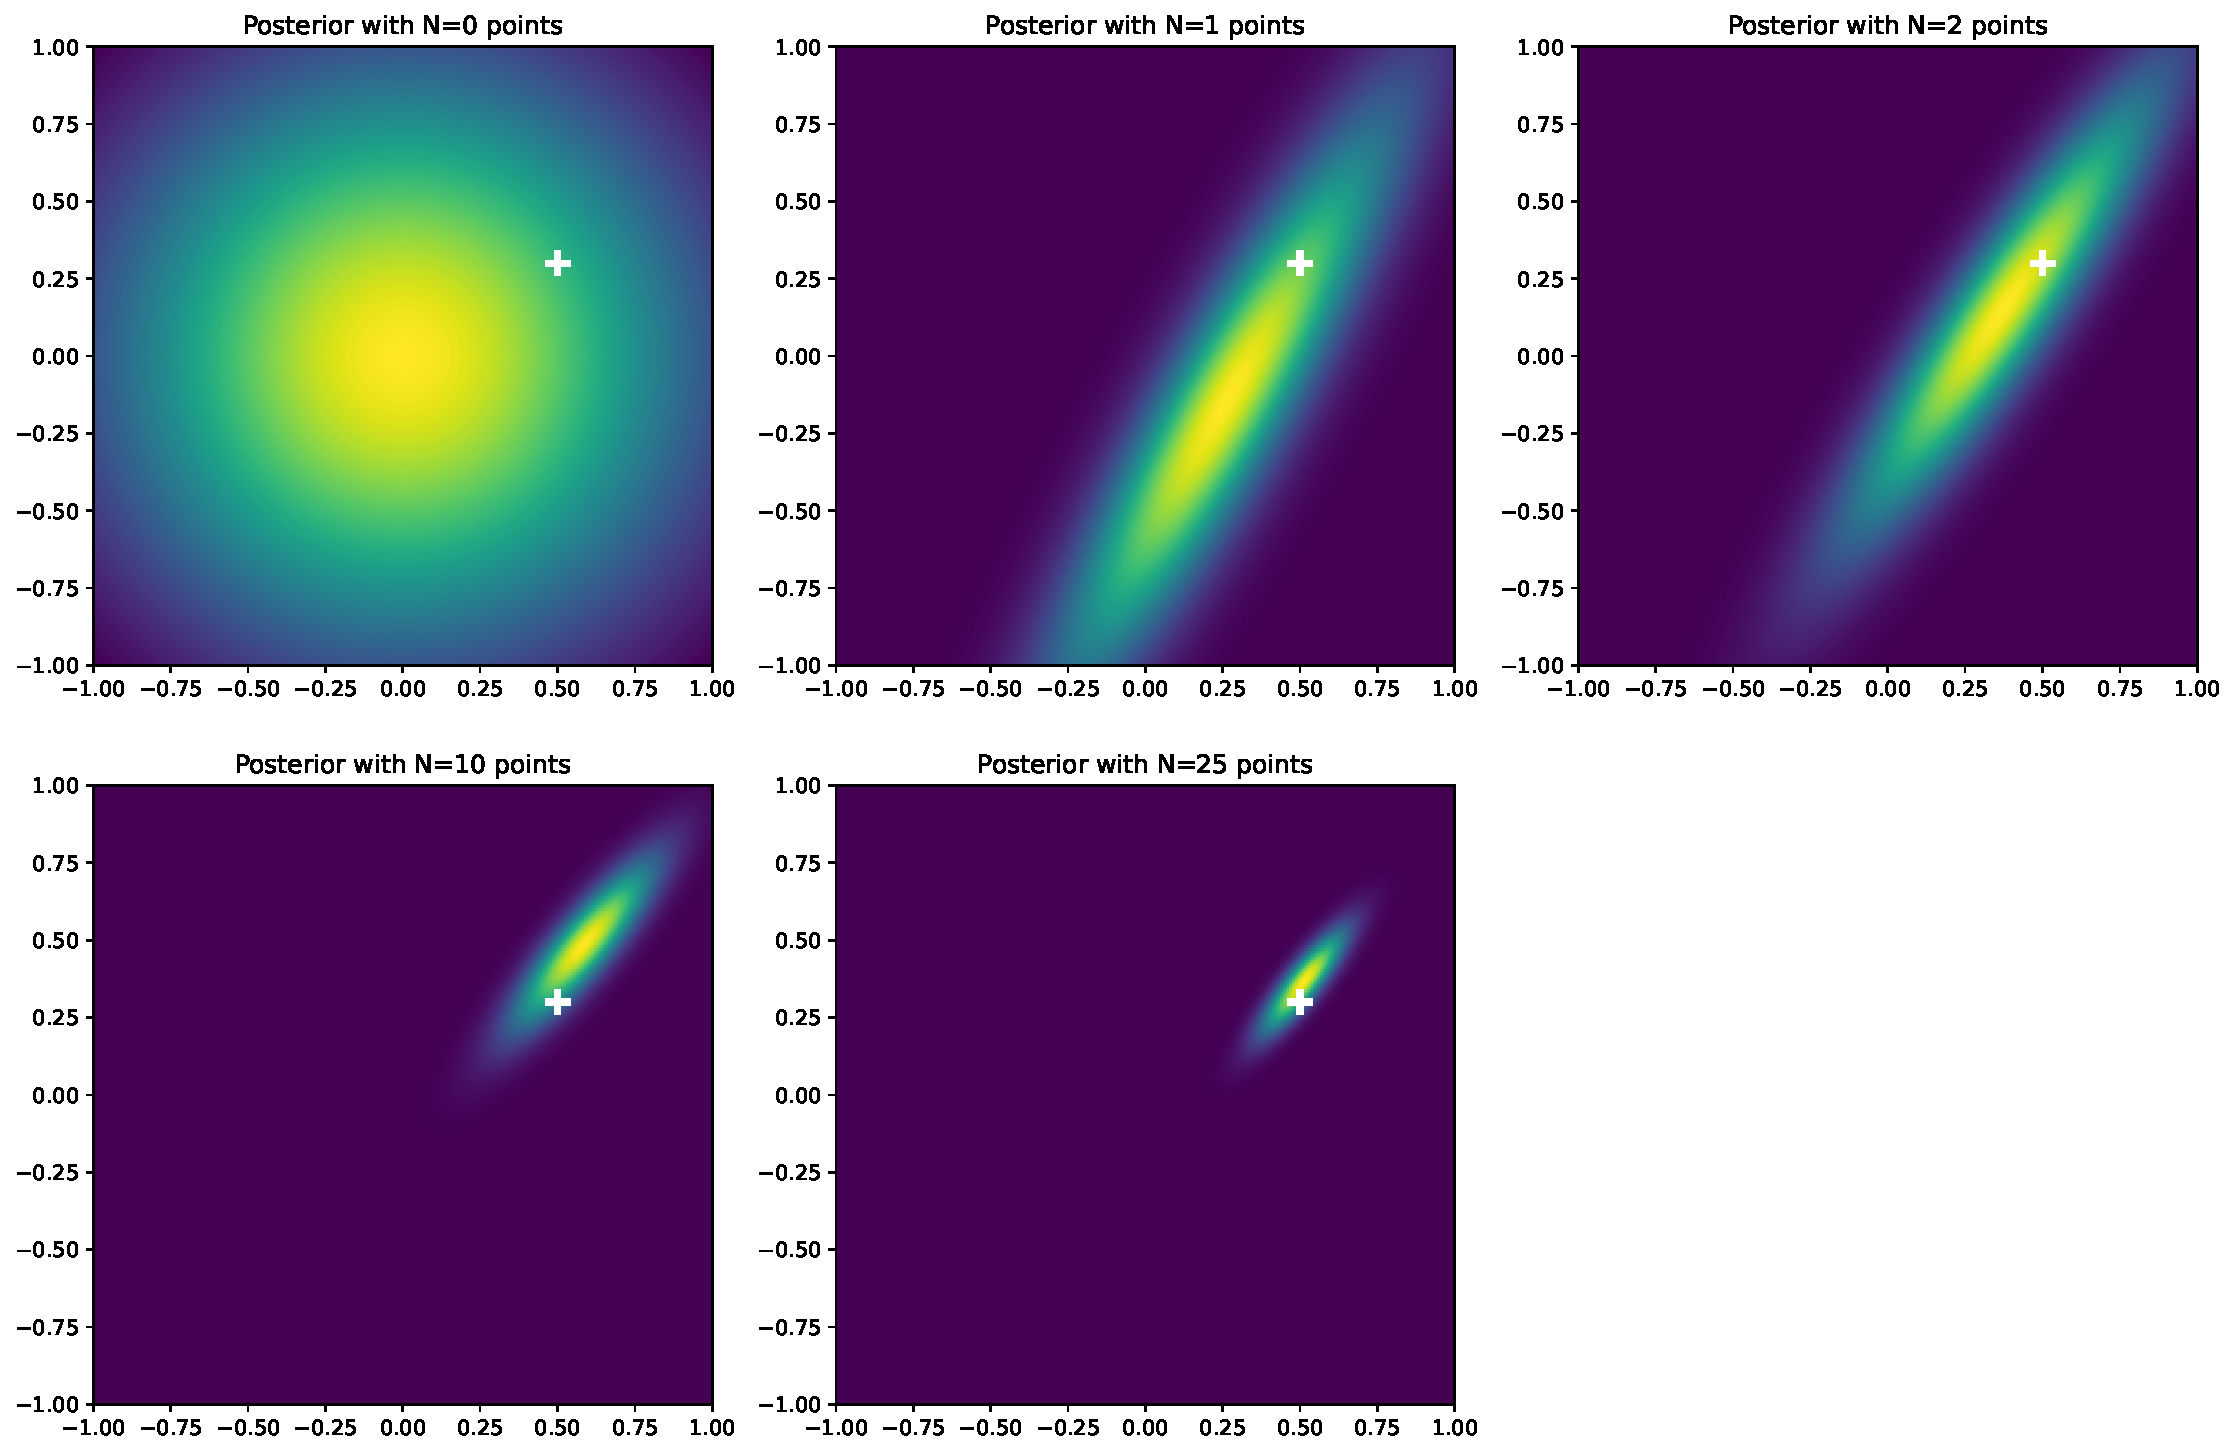
\includegraphics[width=0.95\textwidth]{posterior.pdf}
    \caption{Evolution of a Bayesian posterior distribution with increasing data points: A visual representation of Bayesian inference, depicting how the posterior distribution updates as more data is incorporated. From left to right, the figures show the posterior with $N=0$ (prior distribution), $N=1$, $N=2$, $N=10$, and $N=25$ data points, respectively. The cross mark represents the ground truth.}
    \label{fig:posterior}
\end{figure}

\paragraph*{1.3. Recall and code closed form of the predictive distribution in linear case.}

The closed form of the predictive distribution in linear case is given by:
\[
    p\left(y|x^*; \mathcal{D}, \alpha, \beta\right) = \mathcal{N}\left(y; \mu^T \boldsymbol{\Phi}(x^*), \frac{1}{\beta} + \boldsymbol{\Phi}(x^*)^T \boldsymbol{\Sigma} \boldsymbol{\Phi}(x^*)\right)
\]

where $\mathcal{D}$ is the dataset and $x^*$ a new input.

\paragraph*{1.4. Based on previously defined \texttt{f\_pred()}, predict on the test dataset. Then visualize results using \texttt{plot\_results()} defined at the beginning of the notebook.}

\begin{figure}[!htpb]
    \centering
    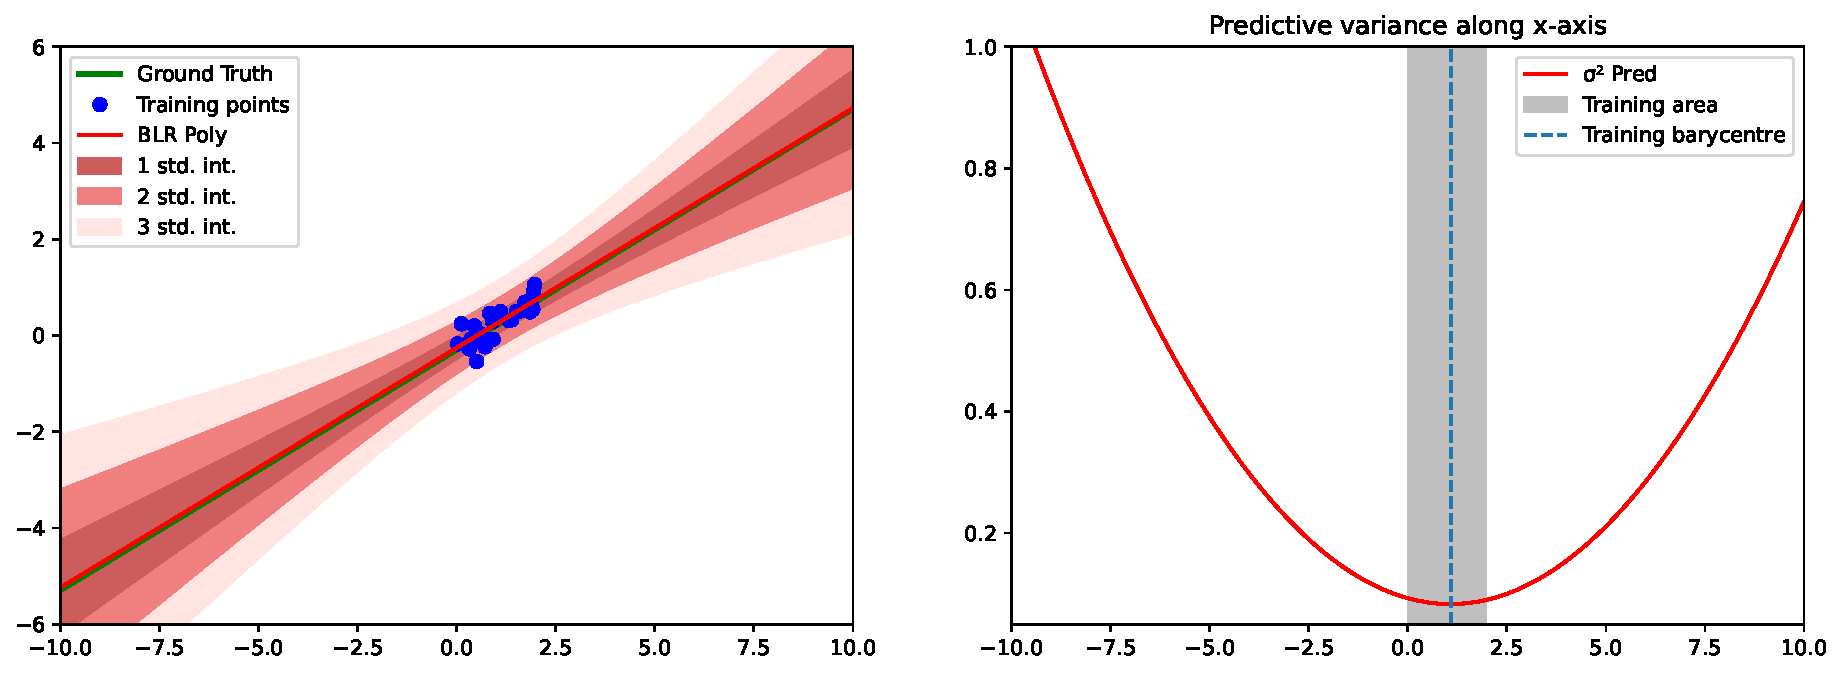
\includegraphics[width=0.95\textwidth]{phi_linear.pdf}
    \caption{The left panel illustrates the Bayesian Linear Regression (BLR) linear fit to the training data (blue points) against the ground truth (green line). The shaded areas represent the predictive uncertainty, with one, two, and three standard deviation intervals shown in progressively lighter shades. The right panel displays the predictive variance $\sigma^2$ across the x-axis. The vertical dashed line indicates the center of the training data.}
    \label{fig:phi_linear}
\end{figure}

\paragraph*{1.5. Analyse these results. Why predictive variance increases far from training distribution? Prove it analytically in the case where $\alpha=0$ and $\beta=1$.}

In the left panel, we can observe that the confidence intervals are narrowest near the cluster of training points. This suggests higher confidence in predictions within this area. As we move away from the center of the training data (towards the extremities of the x-axis), the confidence intervals become wider, indicating increasing uncertainty in the model's predictions.

Looking at the right panel, we notice that the variance remains low in the region where the training data is located (the grey shaded area). This correlates with the tight confidence intervals shown in the left panel. As expected, the predictive variance is lowest near the training barycentre, reflecting greater model certainty in this region due to the presence of more training data points.

As we move away from the training area on either side, the predictive variance increases significantly, which is consistent with the expanding confidence intervals in the left panel. This sharp increase in variance indicates a significant decrease in the model's confidence in its predictions outside the range of the training data. This is a common pattern in regression analysis, as the model has less data to rely on for predictions in these regions. Thus, the Bayesian Linear Regression model offers more reliable predictions within the training data range, with confidence diminishing as predictions move away from this range.\newline

% TODO : continuer la preuve 
With $\alpha = 0, \beta = 1$, the computation of $\Sigma^{-1}$ become 

\begin{align*}
    \Sigma ^{-1} 
        &= 0*Id_3 + 1* \phi ^T \phi = \phi ^T \phi \\ 
        &= \begin{pmatrix}
            1 & \dots & 1 \\
            x_1 & \dots & x_N \\
        \end{pmatrix} \begin{pmatrix}
            1 & x_1 \\
            \vdots & \vdots 
            1 & x_N \\
        \end{pmatrix} \\
        &= \begin{pmatrix}
            N & \sum x_i \\
            \sum x_i & \sum x_i^2
        \end{pmatrix}
\end{align*}

Finally we inverse $ \Phi  $ using the classic formula for $ 2 \times 2 $ matrix 

\[
    \Sigma = \frac{1}{\det \Sigma ^{-1}} \begin{pmatrix}
        \sum x_i^2 & - \sum x_i \\
        - \sum x_i & N
    \end{pmatrix}
    .\]

\paragraph*{Bonus: What happens when applying Bayesian Linear Regression on the following dataset?}

...

\begin{figure}[H]
    \centering
    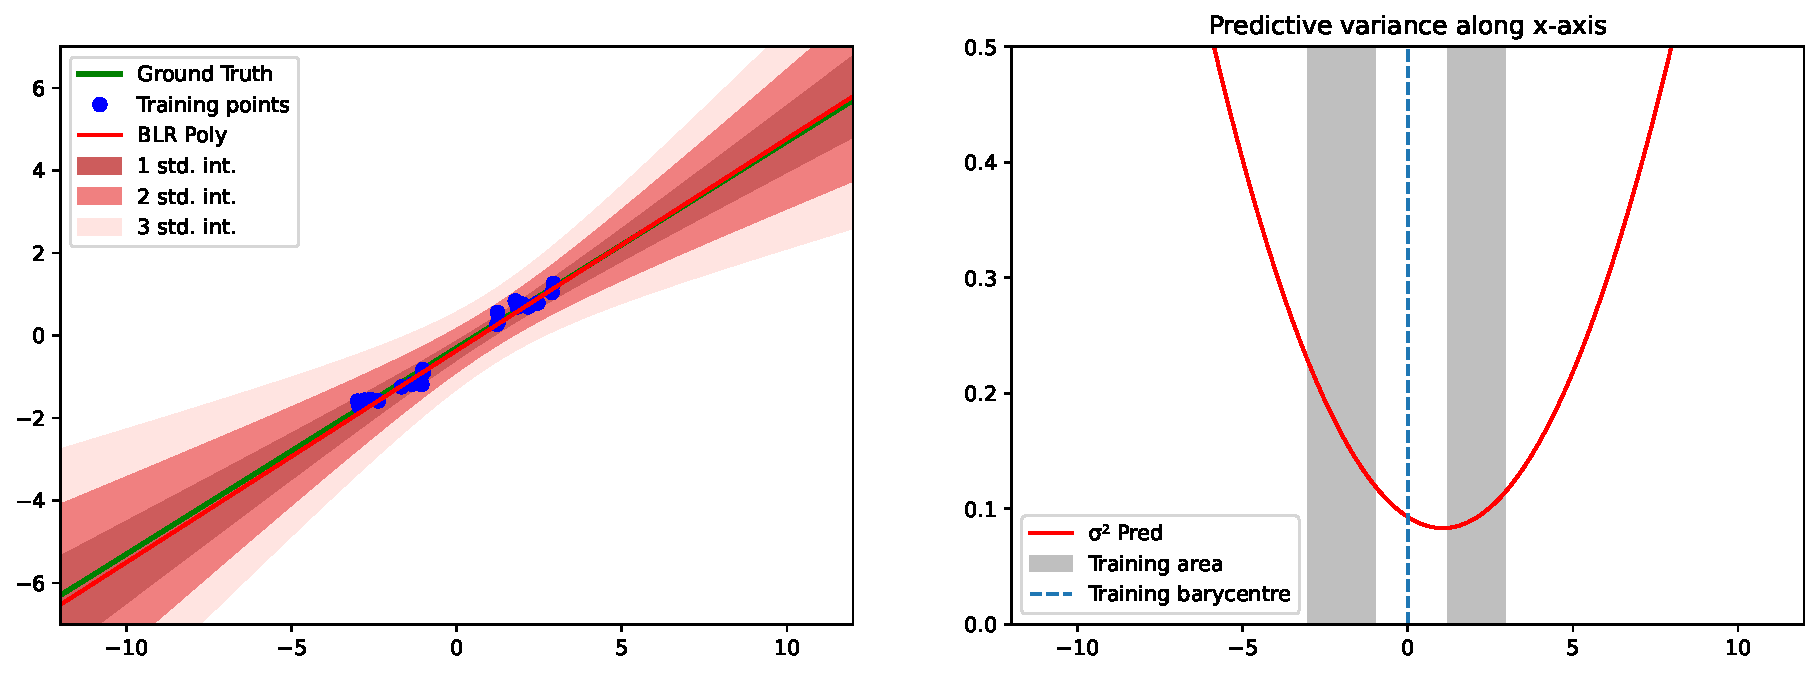
\includegraphics[width=0.95\textwidth]{phi_linear_hole.pdf}
    \caption{Visualization of predictive distribution of a linear dataset featuring a ''hole'': The left panel illustrates the Bayesian Linear Regression (BLR) linear fit to the training data (blue points) against the ground truth (green line). The shaded areas represent the predictive uncertainty, with one, two, and three standard deviation intervals shown in progressively lighter shades. The right panel displays the predictive variance $\sigma^2$ across the x-axis. The vertical dashed line indicates the center of the training data.    }
    \label{fig:phi_linear_hole}
\end{figure}

\section{Non Linear models}

\subsection{Polynomial basis functions}

\paragraph*{2.2. Code and visualize results on sinusoidal dataset using polynomial basis functions. What can you say about the predictive variance?}

...

\begin{figure}[H]
    \centering
    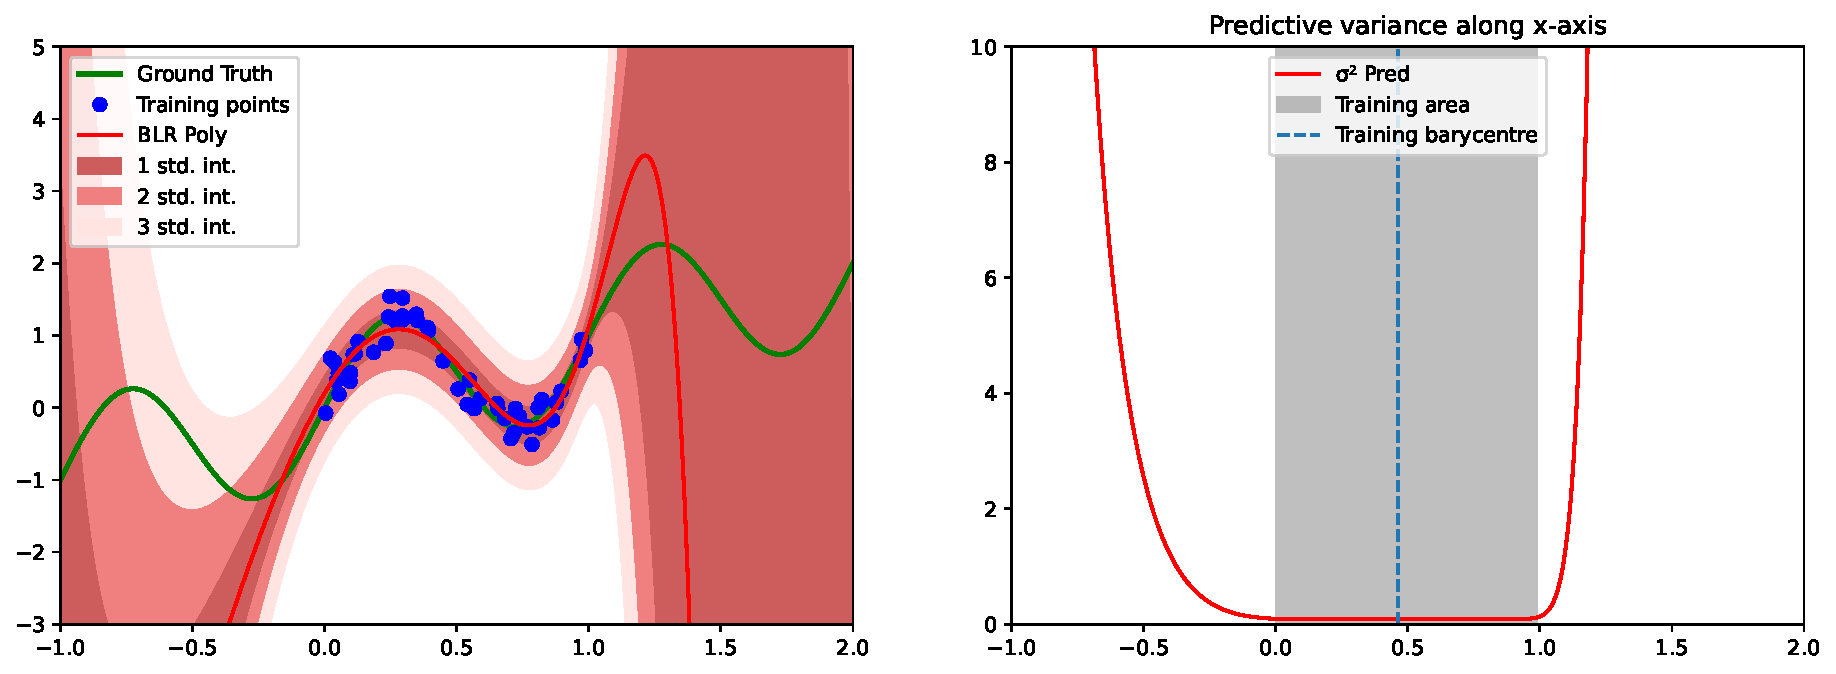
\includegraphics[width=0.95\textwidth]{phi_polynomial.pdf}
    \caption{<caption>}
    \label{fig:phi_polynomial}
\end{figure}

\subsection{Gaussian basis functions}

\paragraph*{2.4. Code and visualize results on sinusoidal dataset using Gaussian basis functions. What can you say this time about the predictive variance?}

...

\begin{figure}[H]
    \centering
    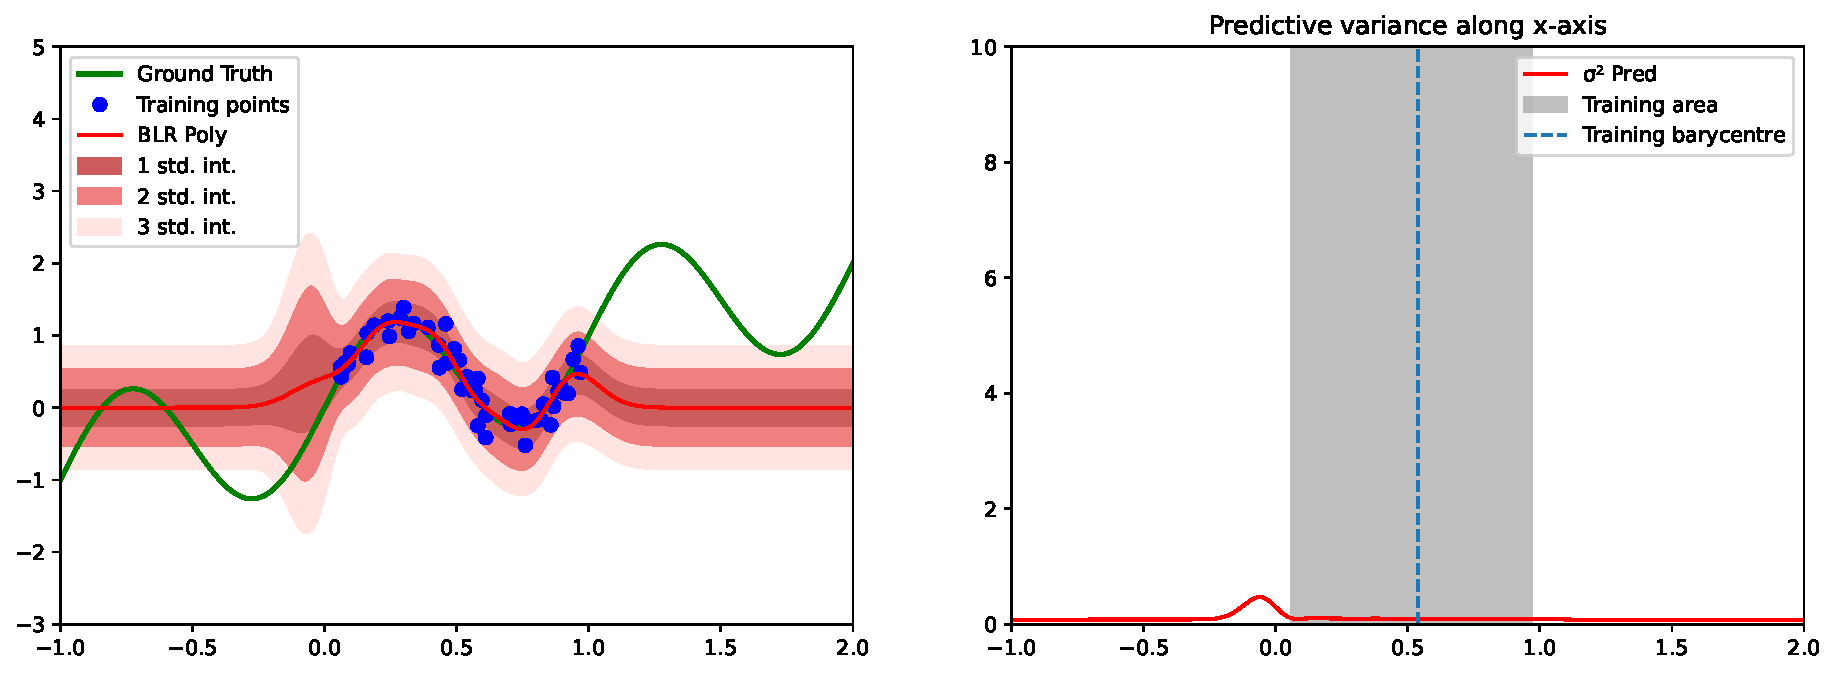
\includegraphics[width=0.95\textwidth]{phi_gaussian.pdf}
    \caption{<caption>}
    \label{fig:phi_gaussian}
\end{figure}

\paragraph*{2.5. Explain why in regions far from training distribution, the predictive variance converges to this value when using localized basis functions such as Gaussians.}


